
\newpage
\section{Návrh}
\label{design}

%TODO spomenut autoencoder

Na základe analýzy problémovej oblasti a existujúcich riešení sme sa rozhodli najprv použiť konvolučnú neurónovú sieť (jej popis a architektúra v kapitole \ref{nn_popis}), čo sa pretavilo aj do prvotných experimentov (kapitola \ref{first_experiments}).

Ďalej sme navrhli autoenkóder k predikcii vizuálnej pozornosti (kapitola \ref{autoencoder_design}) a pokúsili sa použiť už predtrénovaný model VGG-Net siete s autoenkóderom od A. Meyer-a (oba popisované v \ref{object_detection}) na našom predpripravenom datasete.

V závislosti od toho, ktorý model, resp. varianta, sa ukáže byť najpresnejšia sa potom budeme venovať ďalšiemu experimentovaniu s pridávaním dodatočných (top-down) informácií o scéne, akými sú napr. poloha objektov konkrétnych objektov.

\subsection{Dataset}
\label{dataset_description}
Podarilo sa nám nájsť veľké množstvo datasetov, ktoré by sa potencionálne dali použiť pre našu neurónovú sieť, ako napr. 
CAT2000\cite{borji2015cat2000}, NUSEF\footnote{http://mmas.comp.nus.edu.sg/NUSEF.html}, či DUT-OMRON\cite{dut-omron}. Pôvodná myšlienka bola vytiahnuť z každého čo najlepšie vzorky (odstrániť rôzne abstraktné umenie, fraktály, atď.) a dať tak dokopy jeden veľký dataset, na ktorom by bolo možné experimentovať. To sme aj naozaj zrealizovali a takýto dataset použili pri prvotných experimentoch popísaných v kapitole \ref{first_experiments}.

Neskôr sa ale postupne ukázalo, že takto zostrojený dataset zložený z viacerých menších má značné nedostatky. Najväčšími problémami boli:
\begin{itemize}
	\item rozdielna kvalita a veľkosť obrázkov
	\item rozdielna dĺžka pohľadov ľudí na obrázky (2, 5, 10 sekúnd)
	\item rozdielny počet fixácií pre obrázky
	\item rozdielnosť experimentov, pri ktorých sa dáta zbierali (voľné sledovanie, voľné sledovanie s detekciou anomálií, zapamätanie si scény, atď.)
	\item rozdielne zariadenia pre zachytenie fixácií s rôznou vzorkovacou frekvenciou 
\end{itemize}

Z vyššie uvedených dôvodov sme sa preto rozhodli vybrať iba jeden dataset. Voľba padla na DUT-OMRON\cite{dut-omron}, pretože:
\begin{itemize}
	\item obsahuje viac než 5000 obrázkov
	\item obsahuje pohľady 5 ľudí za prvé 2 sekundy
	\item má odstránené extrémy v dátach (z angl. outliers)
	\item viac ako 95\% obrázkov má viac než 50 fixácií
	\item všetky obrázky nemajú iba jeden veľký objekt v strede - t.j. fixácie nie sú stále centrované v tej istej oblasti
	\item veľkosť obrázkov je \textit{400x300}
	\item má dobre štruktúrovane spracované dáta
\end{itemize} 

Z vybraných dát sme si potom predpočítali mapy výraznosti (z angl. saliency maps) použitím fixácií a Gauss-ovho filtra. Mapy výrazností jednotlivých ľudí pre obrázky sme potom spojili dokopy. Takouto úpravou sme potom získali viac než 5000 vzoriek, na ktorých sme ďalej trénovali navrhnuté modely.

\subsection{Konvolučná neurónová sieť}
\label{nn_popis}

Celá architektúra je načrtnutá na schéme na obrázku \ref{my_tensorboard_cnn} vytvorenej pomocou nástroja  TensorBoard\footnote{https://www.tensorflow.org/get\_started/summaries\_and\_tensorboard/}.

Jedná sa o jednoduchú sieť so vstupnou konvolučnou vrstvou pre spracovanie obrázkov. Táto vrstva obsahuje konvolučný filter (veľkosť \textit{5x5}) s aktivačnou funkciou sigmoid. Výstup z nej ďalej pokračuje do vrstvy združovania, kde sa použije operácia MAX s filtrom o veľkosti \textit{2x2} a krokom tiež s veľkosťou \textit{2}. Po nich nasleduje vrstva normalizácie, kde je celý výstup zlúčený do jednej širokej vrstvy. Za ňou sa nachádza plne prepojená vrstva (z angl. fully-connected layer) s aktivačnou funkciou sigmoid a vrstva výpadku (z angl. dropout layer\cite{dropout}), ktorej hodnota (v rozmedzí od 0 do 1) určuje, aké percentuálne množstvo neurónov aj s prepojeniami bude dočasne skrytých. Táto možnosť umožňuje počas učenia sa predchádzať pretrénovaniu. Za vrstvou výpadku už nasleduje iba výstupná vrstva a jej transformácia na 2D maticu, obrázok predstavujúci mapu výraznosti, ktorú chceme dostať.

Aktivačná funkcia sigmoid je použitá najmä preto, že mapa výraznosti je prakticky pravdepodobnostné rozdelenie, t. j. sieť sa snaží predikovať pravdepodobnosti výraznosti každého pixelu. Ako algoritmus učenia sme zvolili štandardný algoritmus spätného šírenia chyby (z angl. backpropagation) s trochu extravagatným FTRL optimizérom.

\begin{figure}[H]
	\begin{center}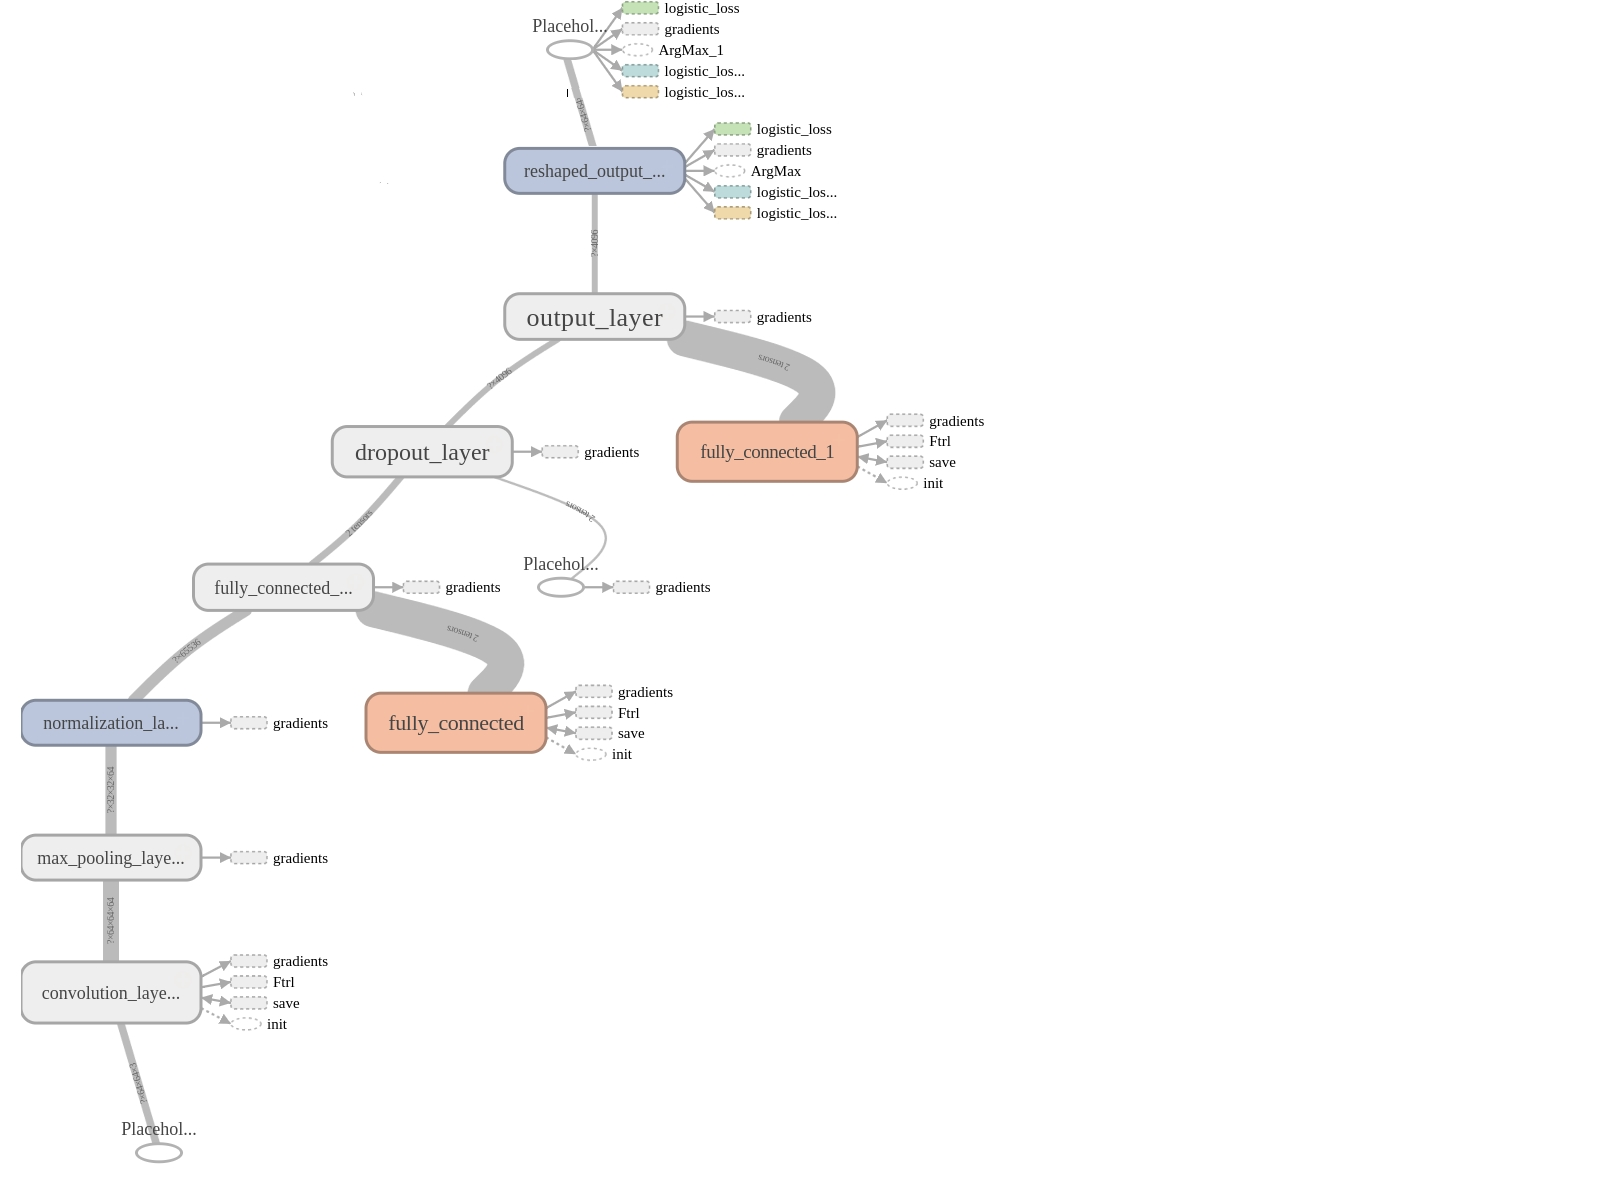
\includegraphics[scale=0.4]{graph-run.jpg}
		\caption[Návrh architektúry neurónovej siete]{
			Diagram reprezentujúci architektúru neurónovej siete, zdola vstupná konvolučná vrstva nasledovaná ostatnými vrstvami siete až po výstupnú, spolu s transformáciou na 2D maticu reprezentujúcu predikovanú mapu výraznosti pre vstupný obrázok
		}\label{my_tensorboard_cnn}
	\end{center}
\end{figure}

\subsection{Autoenkóder}
\label{autoencoder_design}
Ďalším z typov sietí, ktoré sme sa rozhodli otestovať je autoenkóder, konkrétne jeho variácia s konvolučnými vrstvami pre spracovanie obrazu. Jeho úloha je však trochu iná oproti klasickému čo najlepšiemu zrekonštruovaniu vstupu na výstupnej vrstve, miesto toho bude z enkódovaných (komprimovaných dát) predikovať mapy vizuálnej pozornosti. To dosiahneme použitím algoritmu učenia spätného šírenia chyby, kedy ako vstupné dáta budú sieti poskytnuté obrázky a očakávanými výstupmi budú práve mapy vizuálnej pozornosti.

Autoenkóder sa klasicky skladá z dvoch častí, prehľadná štruktúra je zobrazená na obrázku \ref{autoencoder_structure}. Prvou je enkóder, ktorý tvoria 3 konvolučné vrstvy, každá so svojou vlastnou vrstvou združovania, nasledované normalizačnou vrstvou a jednou plne prepojenou vrstvou (z angl. fully-connected layer). Konvolučné vrstvy majú každá filter o veľkosti \textit{3x3} a aktivačnú funkciu ReLU (popísaná v kapitole \ref{activation_functions}), vrstvy združovania podobne ako pri predchádzajúcom type siete používajú operáciu MAX s filtrom o veľkosti \textit{2x2} a krokom rovnako s veľkosťou \textit{2}. Cieľom týchto vrstiev je prakticky extrahovať relevantné črty a vstupný obrázok zmenšiť, resp. komprimovať, čo ďalej zabezpečuje spomínaná normalizačná a plne prepojená vrstva (bez aktivačných funkcií), ktorá už ale vstupný obrázok reprezentuje len ako komprimované jednorozmerné pole. 

Druhou časťou spomínaného autoenkóderu je tzv. dekodér, ktorý sa snaží prakticky zrkadlovými operáciami získať informácie z komprimovaných dát, vďaka čomu je schopný predikovať mapy vizuálnej pozornosti. Jeho vstupnou vrstvou je v podstate výstupná vrstva z enkóderu, ktorej tvar ale musí byť najprv zmenený pre nasledujúce konvolučné vrstvy. Tie sú dokopy štyri, prvé tri konvolučné vrstvy obsahujú filter s veľkosťou \textit{3x3} a aktivačnú funkciu ReLU. Každá z nich je ešte navyše nasledovaná vlastnou vrstvou
prevzorkovania (z angl. upsampling layer), ich cieľom je postupná rekonštrukcia do tvaru vstupného obrázku. Obsahujú vzorkovací faktor 2, na rozdiel od vrstiev združovania v enkóderi však miesto operácie MAX (ktorá dáta, resp. obrázok zmenší) duplikujú riadky a stĺpce poskytnutých dát (obrázka), vďaka čomu sa zväčší o vzorkovací faktor. Posledná výstupná konvolučná vrstva obsahuje filter s veľkosťou \textit{5x5} a aktivačnú funkciu sigmoid. Dátam na nej je ale ešte nutné predtransformovať na 2D maticu, reprezentujúce nami požadované mapy výraznosti. Spomínané trénovanie pomocu algoritmu spätného šírenia chyby využíva Adadelta optimizér (popísaný v časti \ref{optimizers}).

\begin{figure}[H]
	\begin{center}
		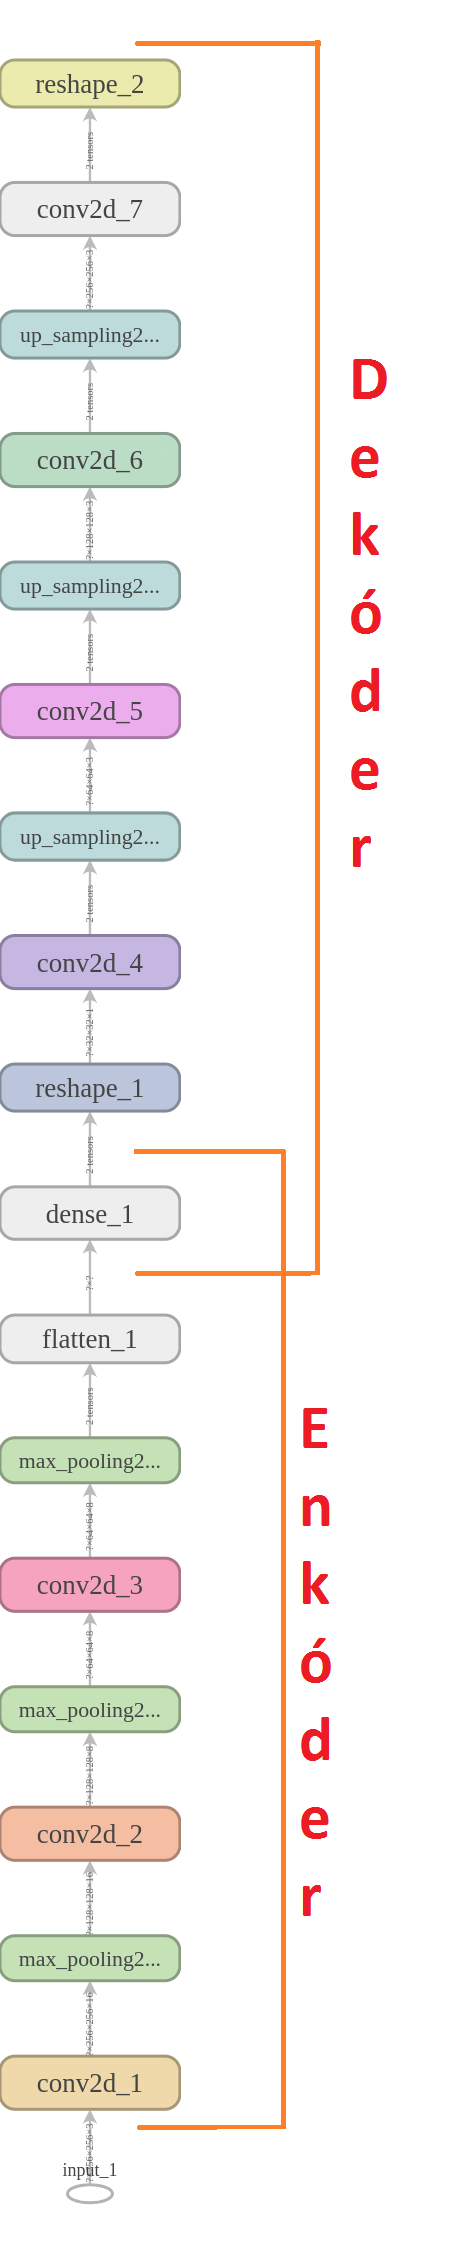
\includegraphics[scale=0.3]{enkoder-dekoder.png}
		\caption[Diagram navrhnutého autoenkóderu]{
			Diagram zobrazujúci architektúru autoenkóderu skladajúceho sa z dvoch častí - enkóderu a dekóderu. Postupne zdola prvá vstupná konvolučná vrstva nasledovaná ostatnými vyššie popísanými vrstvami enkóderu, potom dekóder so svojimi vrstami s konvolúciou a prevzorkovaním až napokon úplne hore výstupná vrstva s predikciou mapy vizuálnej výraznosti. 
		}\label{autoencoder_structure}
	\end{center}
\end{figure}

%TODO autoencoder obrázok

%TODO popisat poriadne transfer learning s autoencoderom s vgg netom

%TODO zhrnutie experimentov s metrikami